
\slidesectionwithgraphic{Course Overview}{images/overview}


\begin{frame}{Course Description | \textbf{Objectives}}

	An advanced C++ seminar \cite{stroustrup2000c++} with supplementary lectures with the following goals:
	
	\begin{itemize}
		\item Deep knowledge in C++ and the STL,
		\item Software development using C++,
		\item Upcoming features of C++17 and C++20,
		\item Using C++ libraries and frameworks
	\end{itemize}
	
	\vfill
	
	\begin{figure}
		
\includegraphics[width=0.09\textwidth]{./images/cpp.pdf}
		\hfill
		
\includegraphics[width=0.17\textwidth]{./images/git.jpg}
		\hfill
		
\includegraphics[width=0.19\textwidth]{./images/cmake.jpg}
		\hfill
		
\includegraphics[width=0.14\textwidth]{./images/openmp.png}
		\hfill
		
\includegraphics[width=0.11\textwidth]{./images/llvm.png}
	\end{figure}
\end{frame}


\begin{frame}[fragile]{Course Description | \textbf{Objectives}}
	
	Entry questionnaire:
	
	% word cloud: xmm, omp parallel for, cmake, left-hand-style, nodiscard, unrestricted, unified memory, thread-local, initialization hell, PCH, GSL, cdecl, universal reference, async, residency, alloca
	% word cloud generator: https://www.wordclouds.com/
	\begin{figure}
		\begin{tikzpicture}
			\node[]{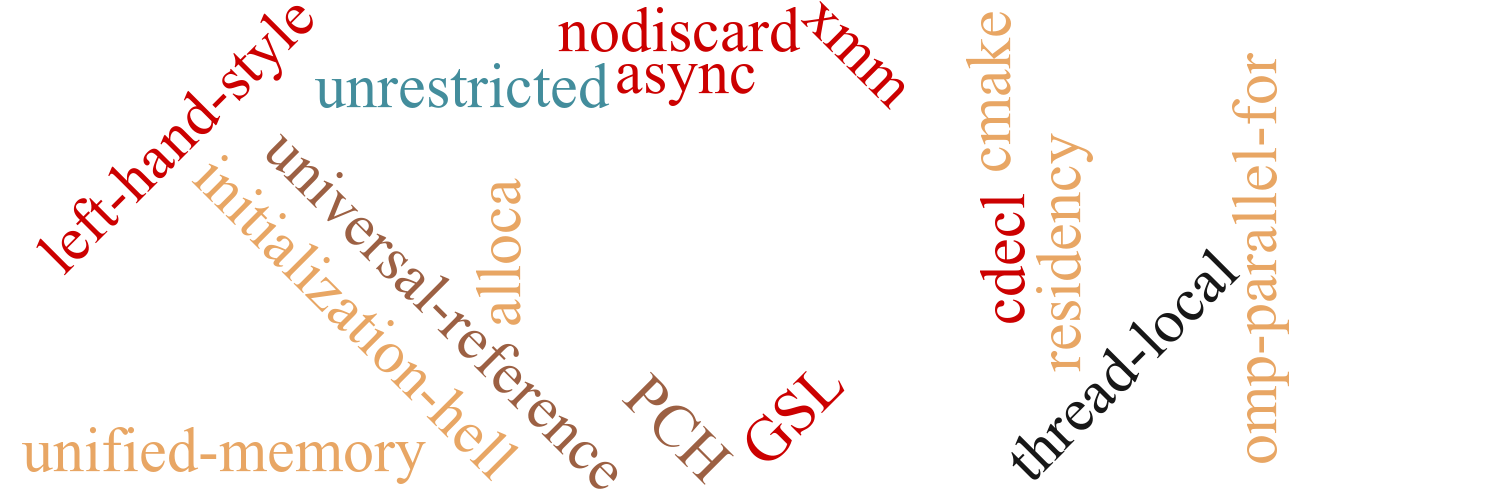
\includegraphics[width=1.0\textwidth]{./images/c++wordcloud.png}};%
			\node[]{
\includegraphics[width=0.16\textwidth]{./images/cpp.pdf}};%
		\end{tikzpicture}
	\end{figure}
	
\end{frame}


\begin{frame}{Course Description | \textbf{Syllabus}}
    
    \twocolumns{0.45}{0.45}
    {
    	The seminar combines practical development in C++ in a team-based software development project and a syllabus of accompanying lectures.
    	
    	\bigskip
    	\bigskip
    	
    	\textbf{Software Development Project}
    	
    	\begin{itemize}
    		%\setlength{\itemsep}{1.5pt}
    		\item A C++ software project,
    		\item in teams up to 4 students,
    		\item three presentations
	    		\begin{itemize}
	    			\item goal presentation
			    	\item intermediate results
			    	\item final presentation
	    		\end{itemize}
    		\item with focus on technical challenges and solutions
    	\end{itemize}
    }
    {
    	\textbf{Lecture Syllabus}
    	
        \begin{itemize}
        	%\setlength{\itemsep}{1.5pt}
            \item Development Guidelines
            \item Best Practices, Common Pitfalls
            \item Cross-Platform Development
            \item Exceptions
            \item Language Internals
            \item Compiler Internals
            \item Vectorization
            \item Multithreading / Parallelization
            \item Heterogeneous Computing
	        \item Foreign Language Integration
	        \item Upcoming Features
	        \item Software Project Setup
        \end{itemize}
    }

\end{frame}


\begin{frame}[fragile]{Course Description | \textbf{Organizational}}

	\medskip
	\begin{tabular}{r|lr}

        \blueify{Course Classification} & Modules ITSE-*, SAMT-*, HCGT-* & \grayout{New HPI Master Program} \\
			& Modules ITSE, HCT, SAMT & \grayout{Previous HPI Master Program\bigskip} \\

		\blueify{Credit Points} & \multicolumn{2}{l}{Project Seminar (6 ETCS)} \bigskip\\
		
		\blueify{Course Meeting Times} & \multicolumn{2}{l}{Monday, 13:30-15:00 HS3}\bigskip\\
		
		\blueify{Course Materials} & \multicolumn{2}{l}{Lecture Slides (pdf)} \\
			& \multicolumn{2}{l}{Supplementary Documents (pdf)} \\
			& \multicolumn{2}{l}{Hands-on Code (zip)} \\
			& \multicolumn{2}{l}{\url{https://moodle.hpi3d.de} (pw: shegalkin)} \bigskip\\

		\blueify{Instructor} & Prof. Dr. Jürgen Döllner & \bigskip \\
		
		\blueify{Tutors}
			& Willy Scheibel & \grayout{willy.scheibel@hpi.de} \\
			& Jan Ole Vollmer & \grayout{jan.vollmer@hpi.de}

	\end{tabular}

\end{frame}


\begin{frame}[fragile]{Course | \textbf{Frameworks and Tools}}
	
	\bigskip

	\begin{tabular}{r|l}
				
		\blueify{Architecture and Platform} & x86 or x86-64 (preferred) on either Windows, Linux, or macOS \bigskip\\
		
		\blueify{Project Setup} & CMake for cross-platform project setup \\ 
		& \url{https://cmake.org} \bigskip\\
		
		\blueify{Debugger} & GDB or Debugging Tools for Windows \bigskip\\
		
		\blueify{Coding Guidelines} & \url{https://isocpp.github.io/CppCoreGuidelines/CppCoreGuidelines} \\
			& \grayout{\url{https://google.github.io/styleguide/cppguide.html}} \\
			& \grayout{\url{https://cginternals.github.io/guidelines}}\\
		
	\end{tabular}
			
\end{frame}


\begin{frame}{Course | \textbf{Assessment}}

    \vfill
    \twocolumns{0.65}{0.3}
    {
        The assessment for this course includes practical work, involving software development, and the oral presentations.
        \bigskip
    
        \textbf{Grading}
        \begin{itemize}
            \item 40\% oral presentations (10\%, 10\%, 20\%)
            \item 50\% software development
            \item 10\% project publication or submission
        \end{itemize}
    }
    {
        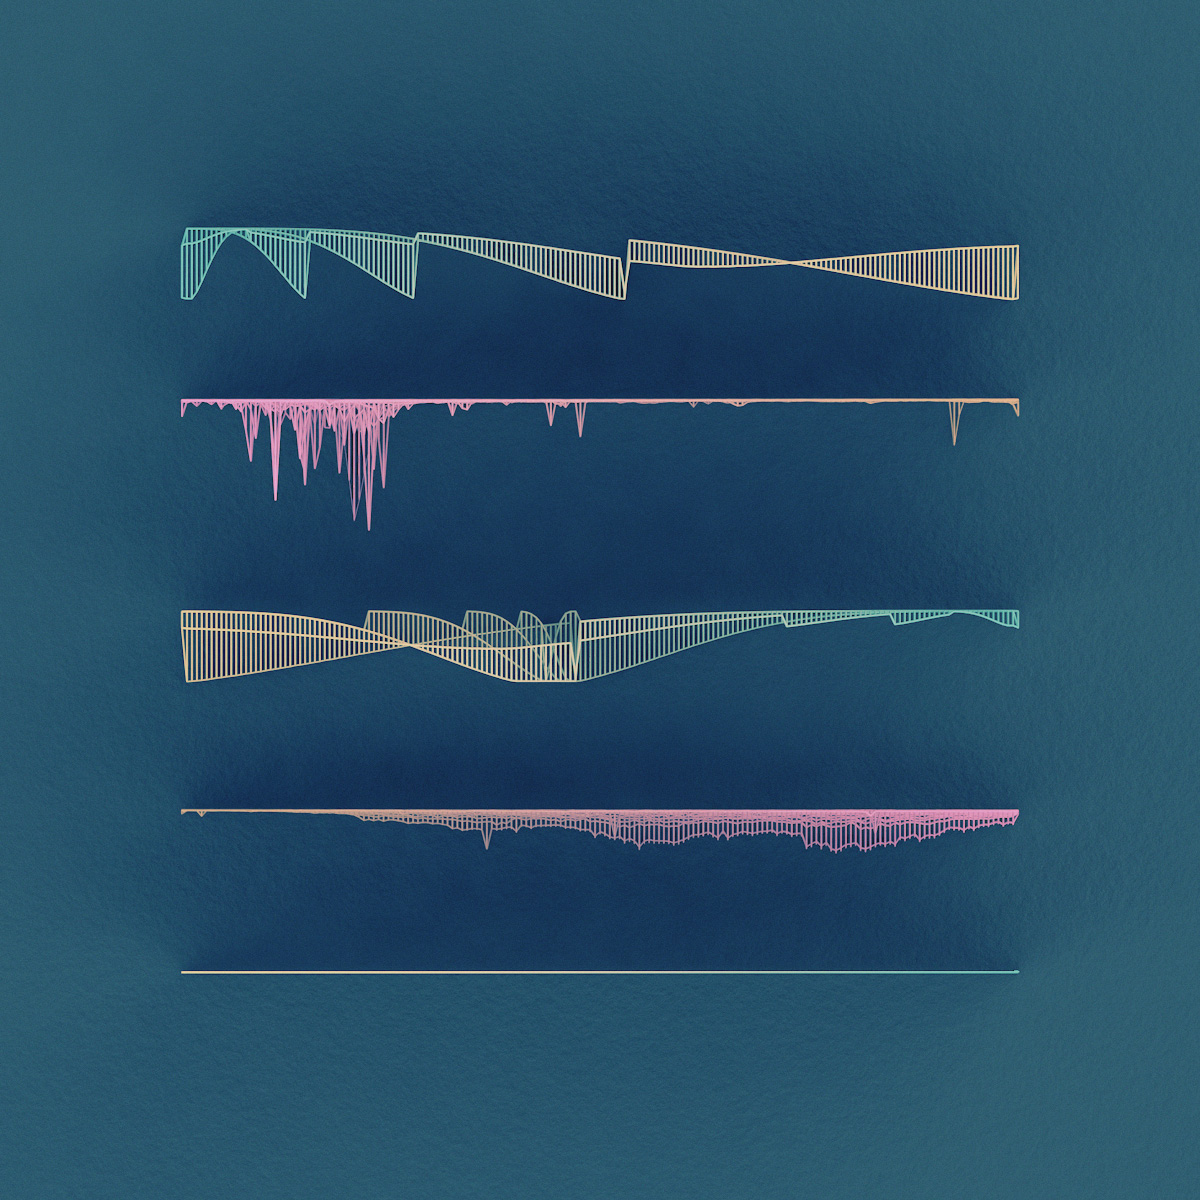
\includegraphics[width=\textwidth]{images/scoring}   
    }
    \vfill

\end{frame}


\begin{frame}{Course | \textbf{Literature}}
    
    \twocolumns{0.35}{0.6}
    {
        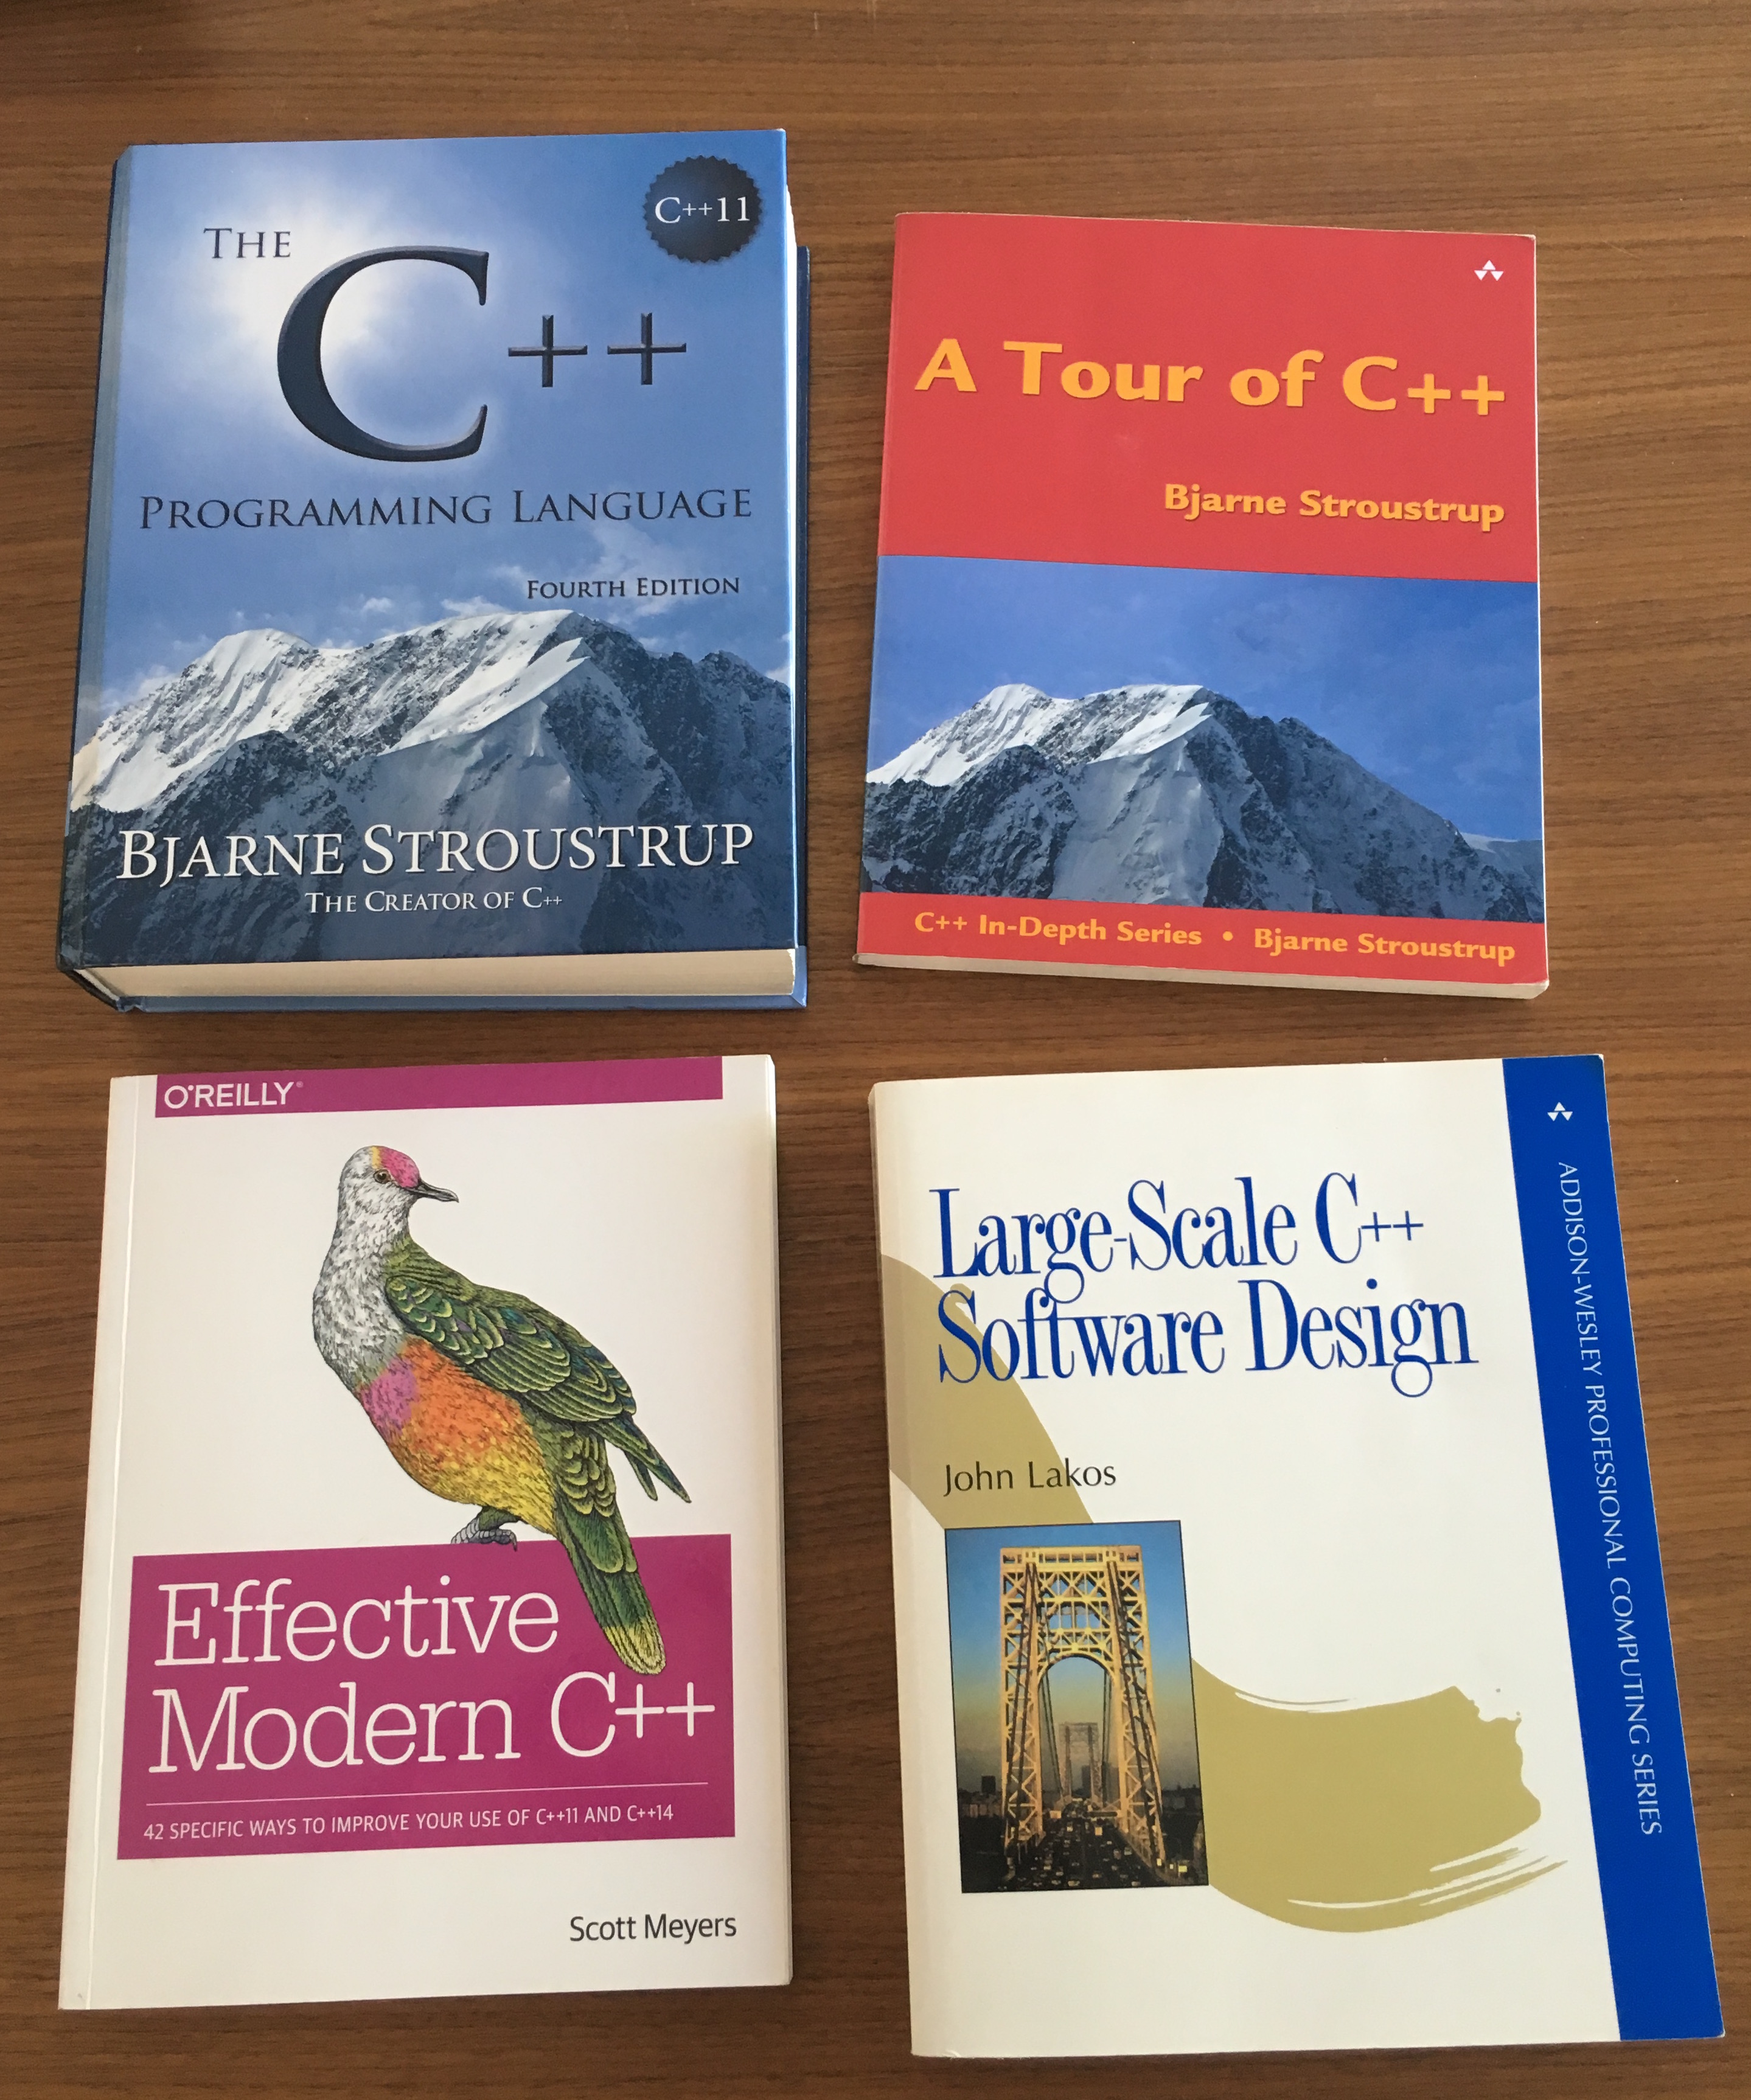
\includegraphics[width=\textwidth]{images/buecher}
    }
    {
    	\begin{itemize}
            \item Bjarne Stroustrup: \enquote{The C++ Programming Language},\\Addison-Wesley Professional, ISBN 978-0321563842
            \medskip
            \item Bjarne Stroustrup: \enquote{A Tour of C++},\\Addison-Wesley Professional, ISBN 978-0321958310
            \medskip
            \item Scott Meyers: \enquote{Effective Modern C++},\\O'Reilly Media, ISBN 978-1491903995
            \medskip
            \item John Lakos: \enquote{Large-Scale C++ Software Design},\\Addison-Wesley Professional, ISBN 978-0201633627
        \end{itemize}
    }

\end{frame}


\begin{frame}{Course | \textbf{Literature}}
    
    \twocolumns{0.35}{0.6}
    {
        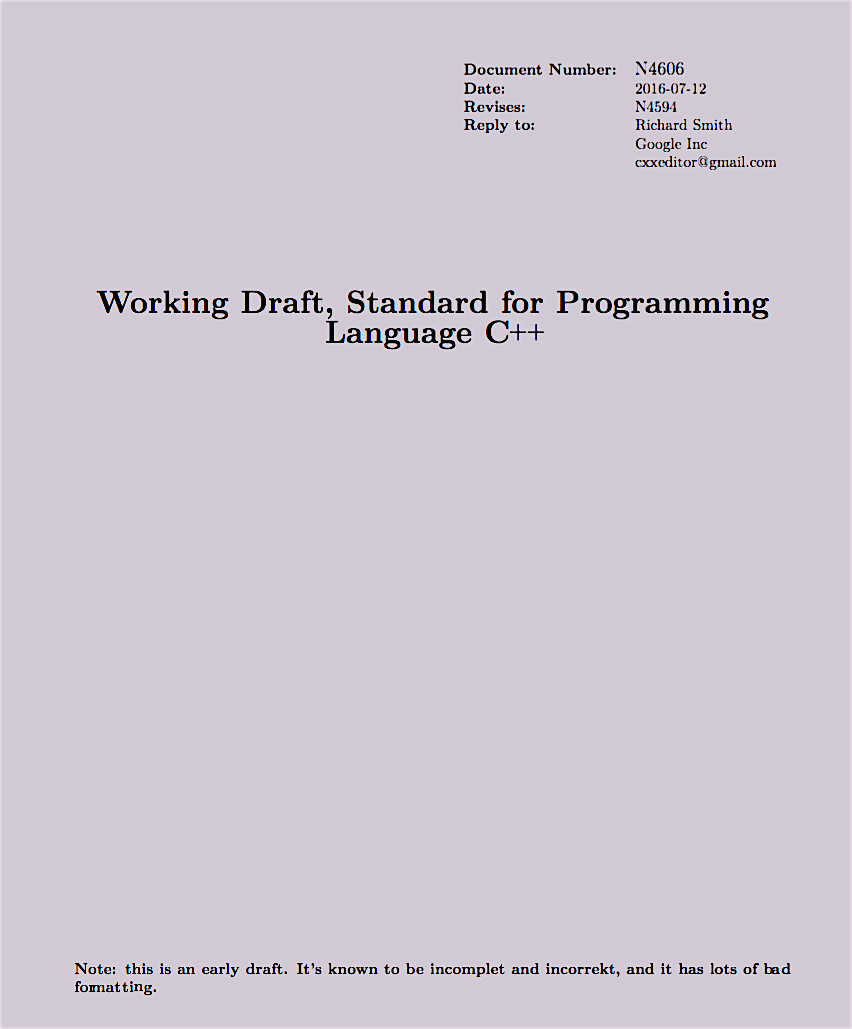
\includegraphics[width=\textwidth]{images/iso4606}
    }
    {
        \begin{itemize}
            \item ISO International Standard ISO/IEC 
            – Programming Language C++, Working Drafts C++ 17 \\
            PDF at \url{https://isocpp.org/std/the-standard}
        \end{itemize}
    }

\end{frame}